\begin{figure}[ht!]
	\centering
	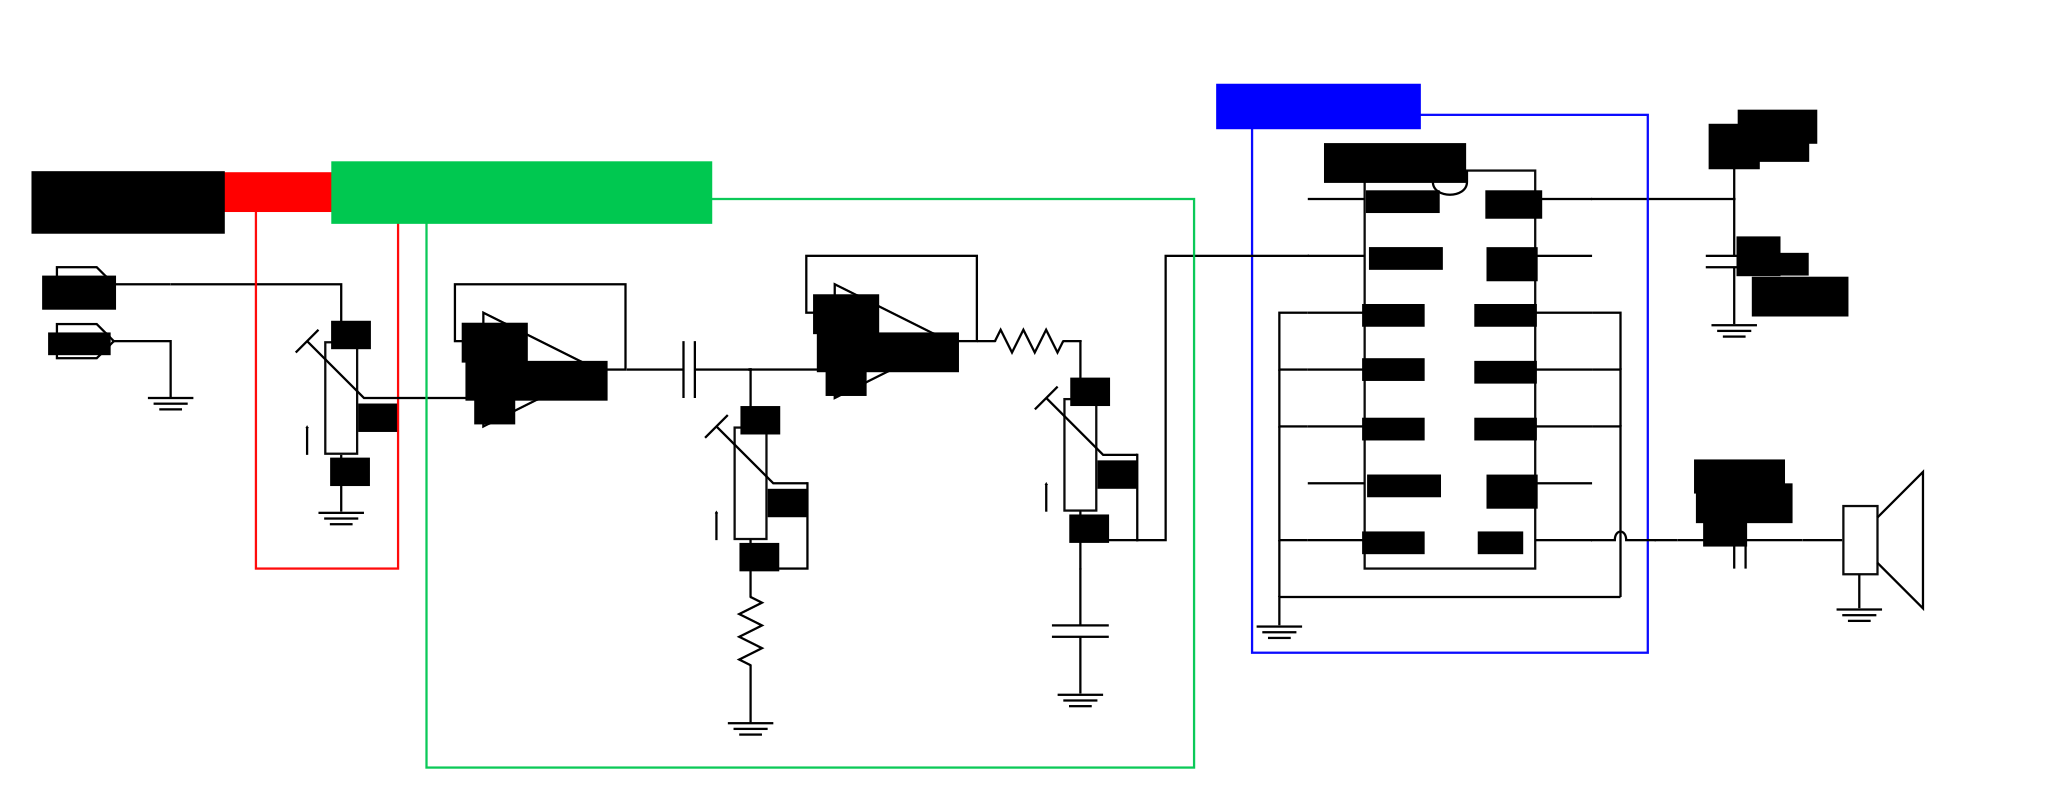
\includegraphics[width=\textwidth]{schematics}
	\caption{Schématique du circuit.}
	\label{fig2:schematics}
\end{figure}

Le schématique du circuit modifié est présenté à la Figure \ref{fig2:schematics}. En partant de la gauche, le signal d'entrée fourni par le câble jack à la borne IN1 passe d'abord dans le bloc de filtrage. Les filtres ont été implémentés sur base de topologies passe-haut et passe-bas passives, c'est-à-dire qu'elles n'utilisent pas d'amplificateur opérationnel. Pour éviter que l'impédance d'entrée (resp. sortie) des blocs suivants (resp. précédents) ait un impact sur le comportement des filtres, ceux-ci sont isolés du reste du circuit par des montages suiveurs, à savoir un amplificateur opérationnel avec une rétroaction unitaire sur la borne négative.Le signal est ensuite transmis au bloc de distorsion (de type overdrive/clipper), inspiré de la pédale appelée \textit{Dan Armstrong's Blue Clipper}. Le détail de ce circuit est présenté à la Figure \ref{fig3:clipper}. Ce bloc inclus également le contrôle du volume, implémenté par un diviseur résistif. Enfin, le signal est amplifié puis transmis au haut-parleur.